\documentclass[10pt,xcolor=pdflatex]{beamer}
\usepackage{newcent}
\usepackage[utf8]{inputenc}
\usepackage[czech]{babel}
\usepackage{hyperref}
\usepackage{fancyvrb}
%\usetheme[]{FIT}
\usetheme[CZlogo]{FIT} % CZ logo

%%%%%%%%%%%%%%%%%%%%%%%%%%%%%%%%%%%%%%%%%%%%%%%%%%%%%%%%%%%%%%%%%%
\title[Obhajoba semestrálního projektu]{Části webové stránky šifrované pomocí GPG}
\newcommand{\czuv}[1]{\quotedblbase #1\textquotedblleft}
\author[]{Jiří Matějka}

% \institute[]{Brno University of Technology, Faculty of Information Technology\\
% Bo\v{z}et\v{e}chova 1/2. 612 66 Brno - Kr\'alovo Pole\\
% login@fit.vutbr.cz}

% CZ verzia
\institute[]{Vysoké učení technické v Brně, Fakulta informačních technologií\\
Božetěchova 1/2 612 66 Brno\\
xmatej52@stud.fit.vutbr.cz}


\date{21. 1. 2020}
%\date{\today}
%\date{} % bez data

%%%%%%%%%%%%%%%%%%%%%%%%%%%%%%%%%%%%%%%%%%%%%%%%%%%%%%%%%%%%%%%%%%

\begin{document}

\frame[plain]{\titlepage}

\begin{frame} 
    \frametitle{Co implementuji?}
    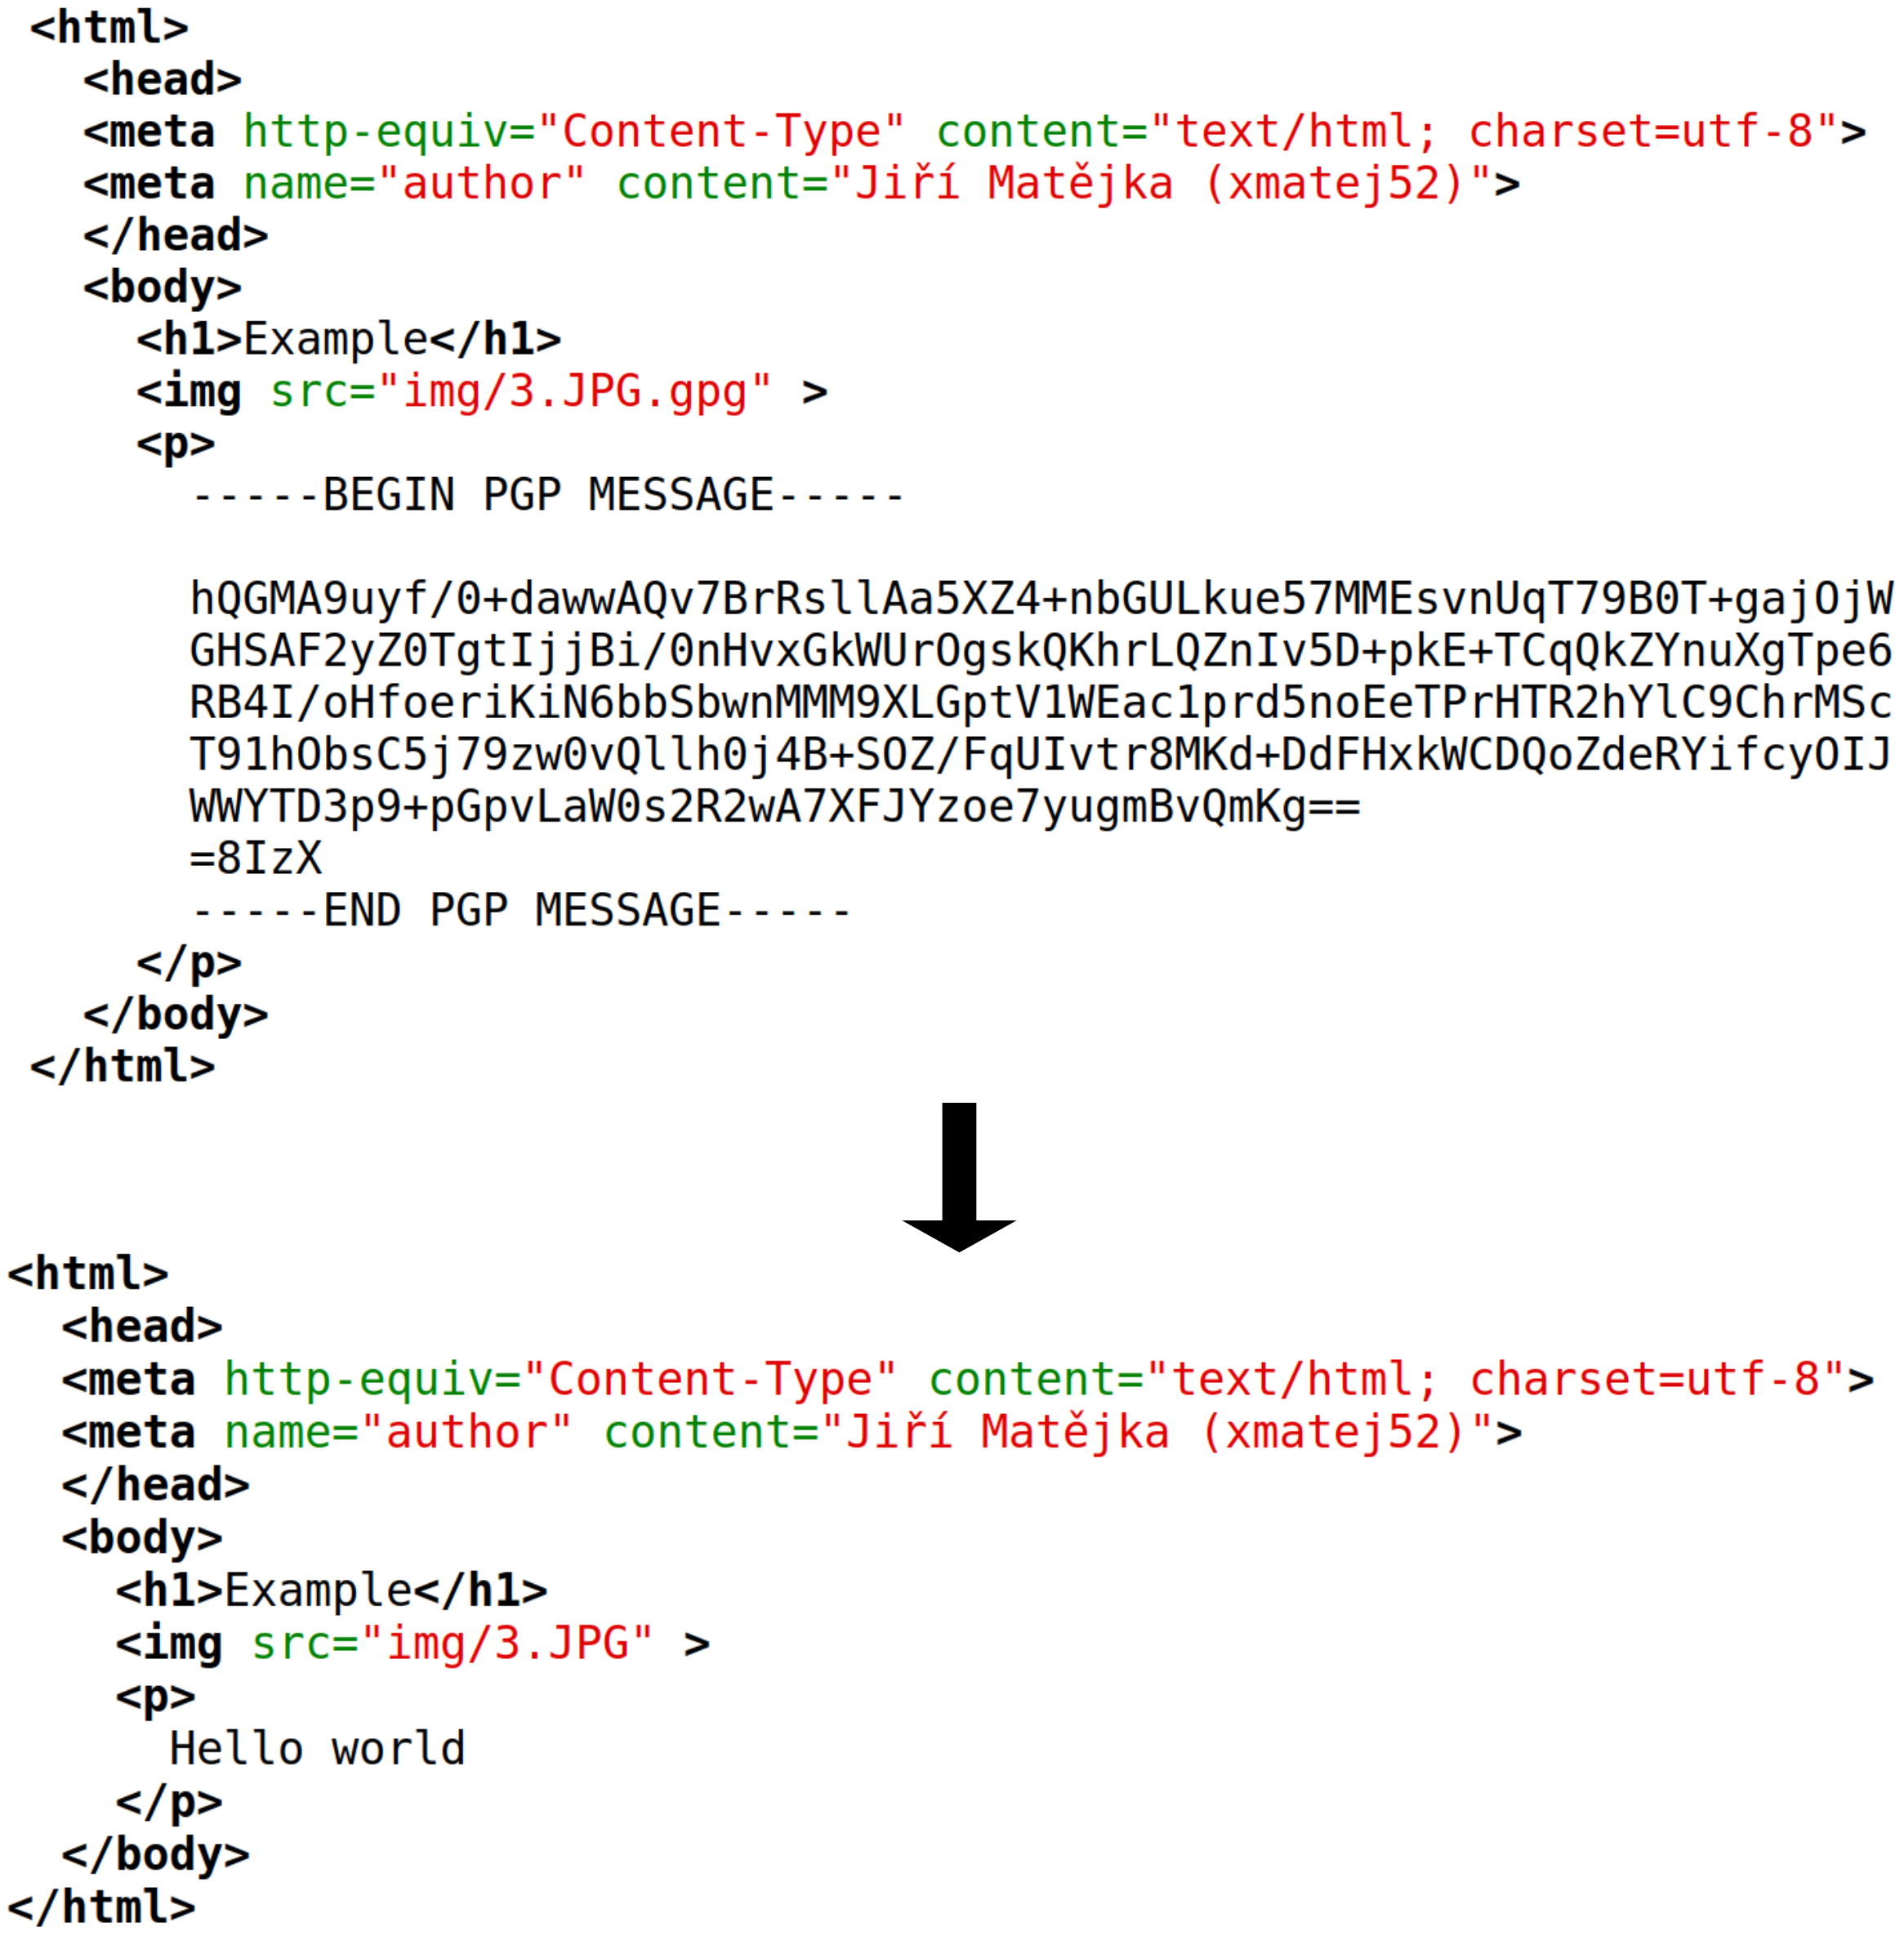
\includegraphics[width=\textwidth,height=0.9\textheight,keepaspectratio]{img/example.png}
\end{frame}

\begin{frame}
    \frametitle{Návrh rozšíření}
    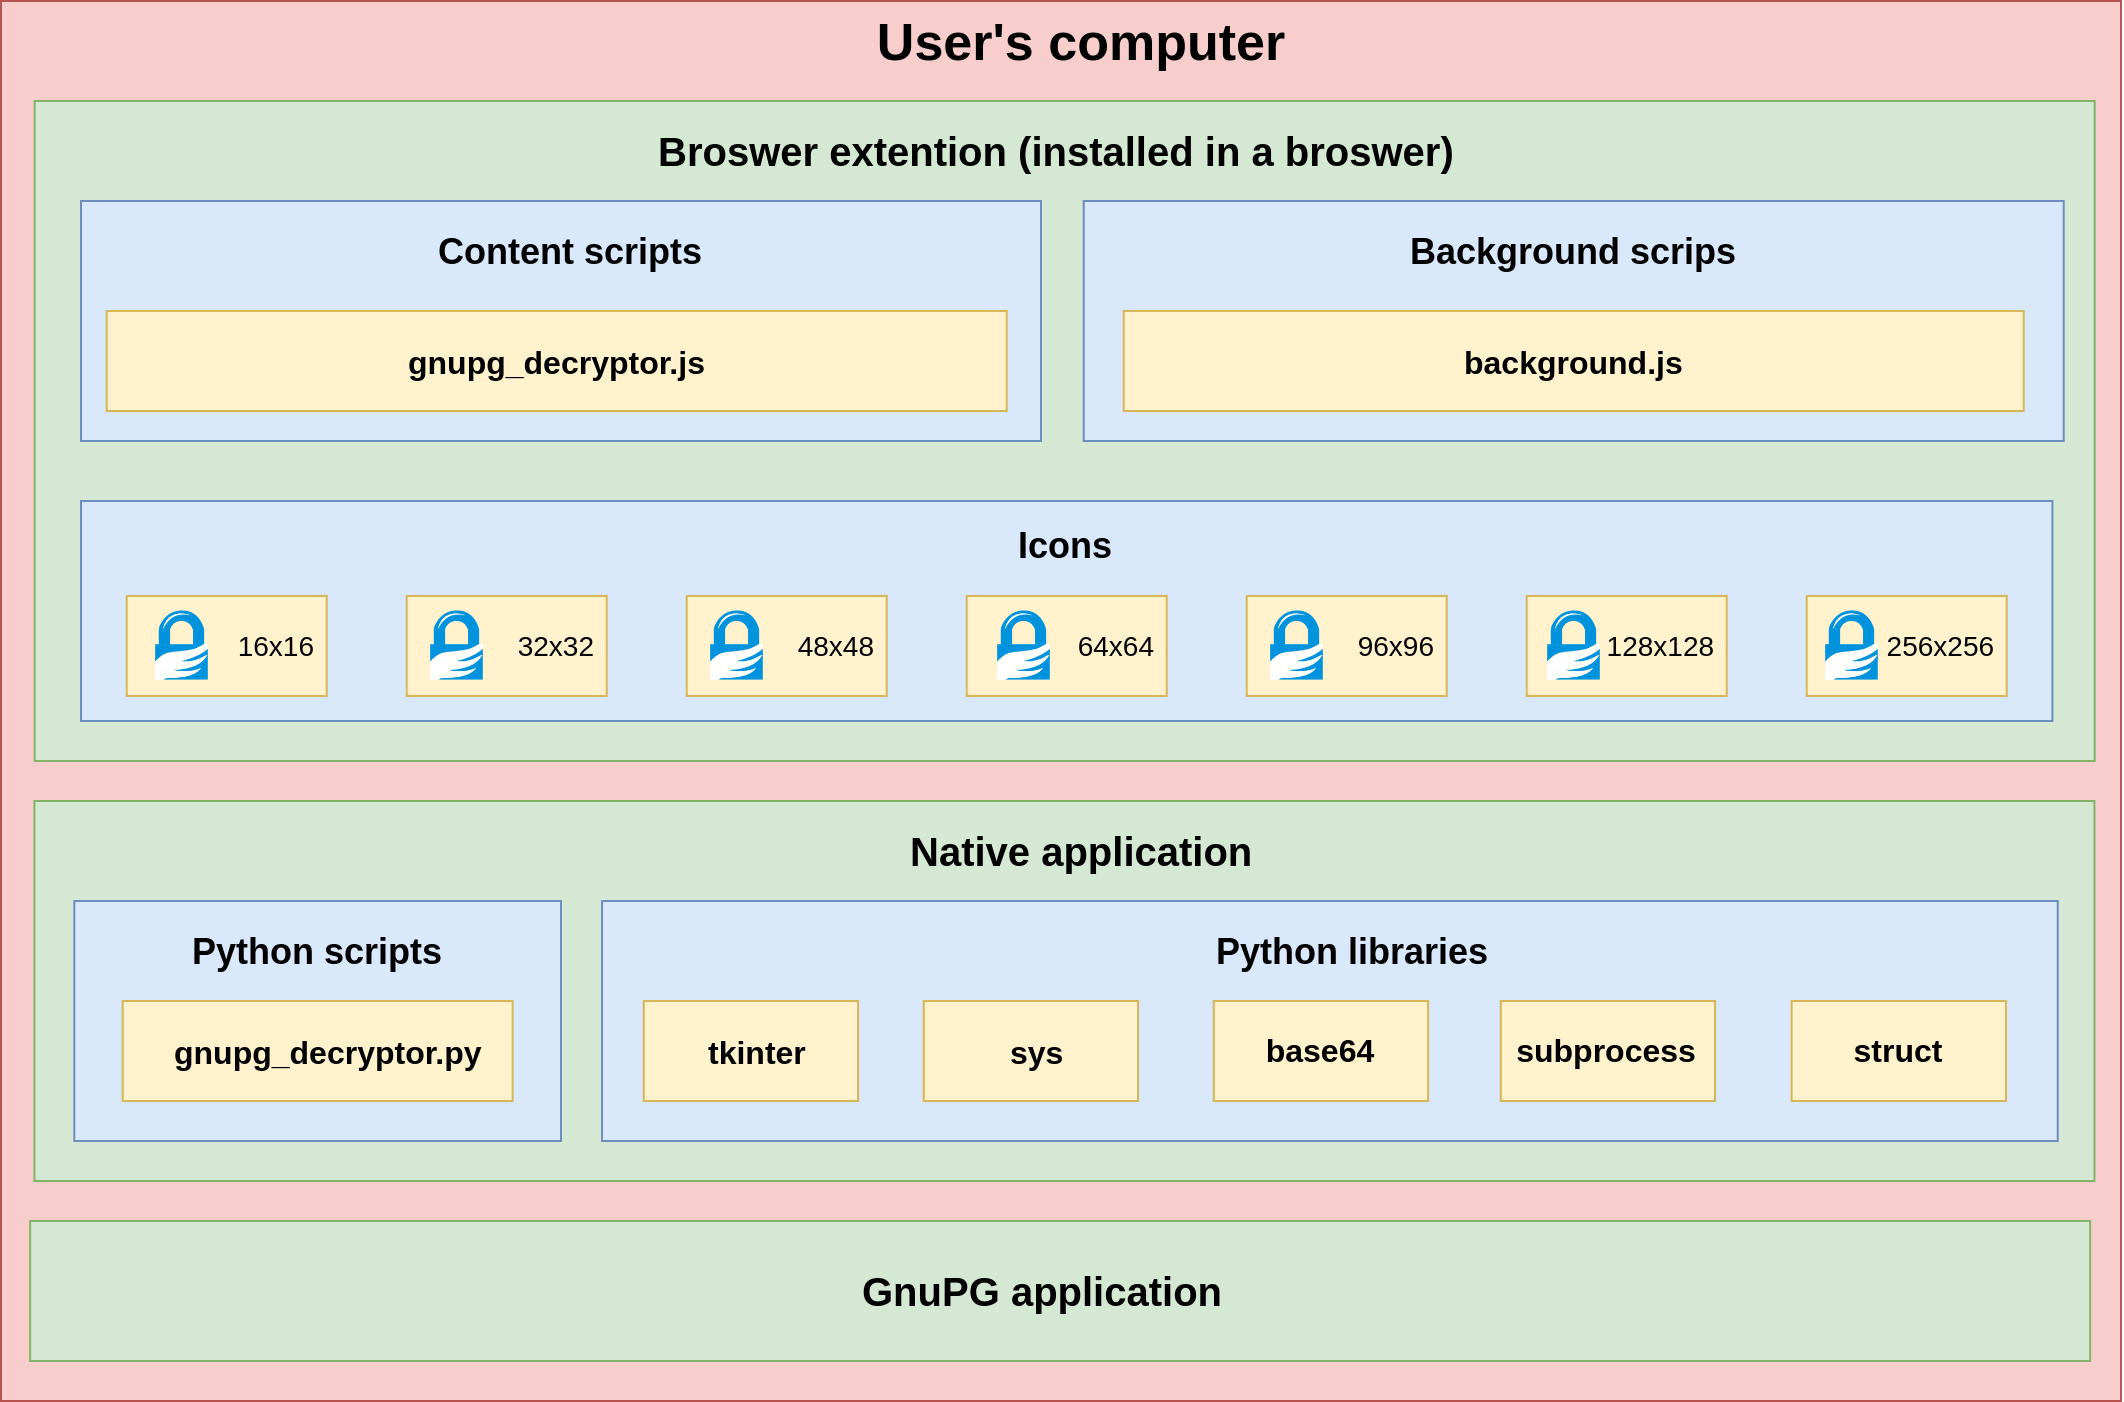
\includegraphics[width=\textwidth]{../obrazky-figures/prototype-GnuPG_Decryptor.png}
\end{frame}

\begin{frame}
    \frametitle{Komunikace rozšíření a nativní aplikace}
    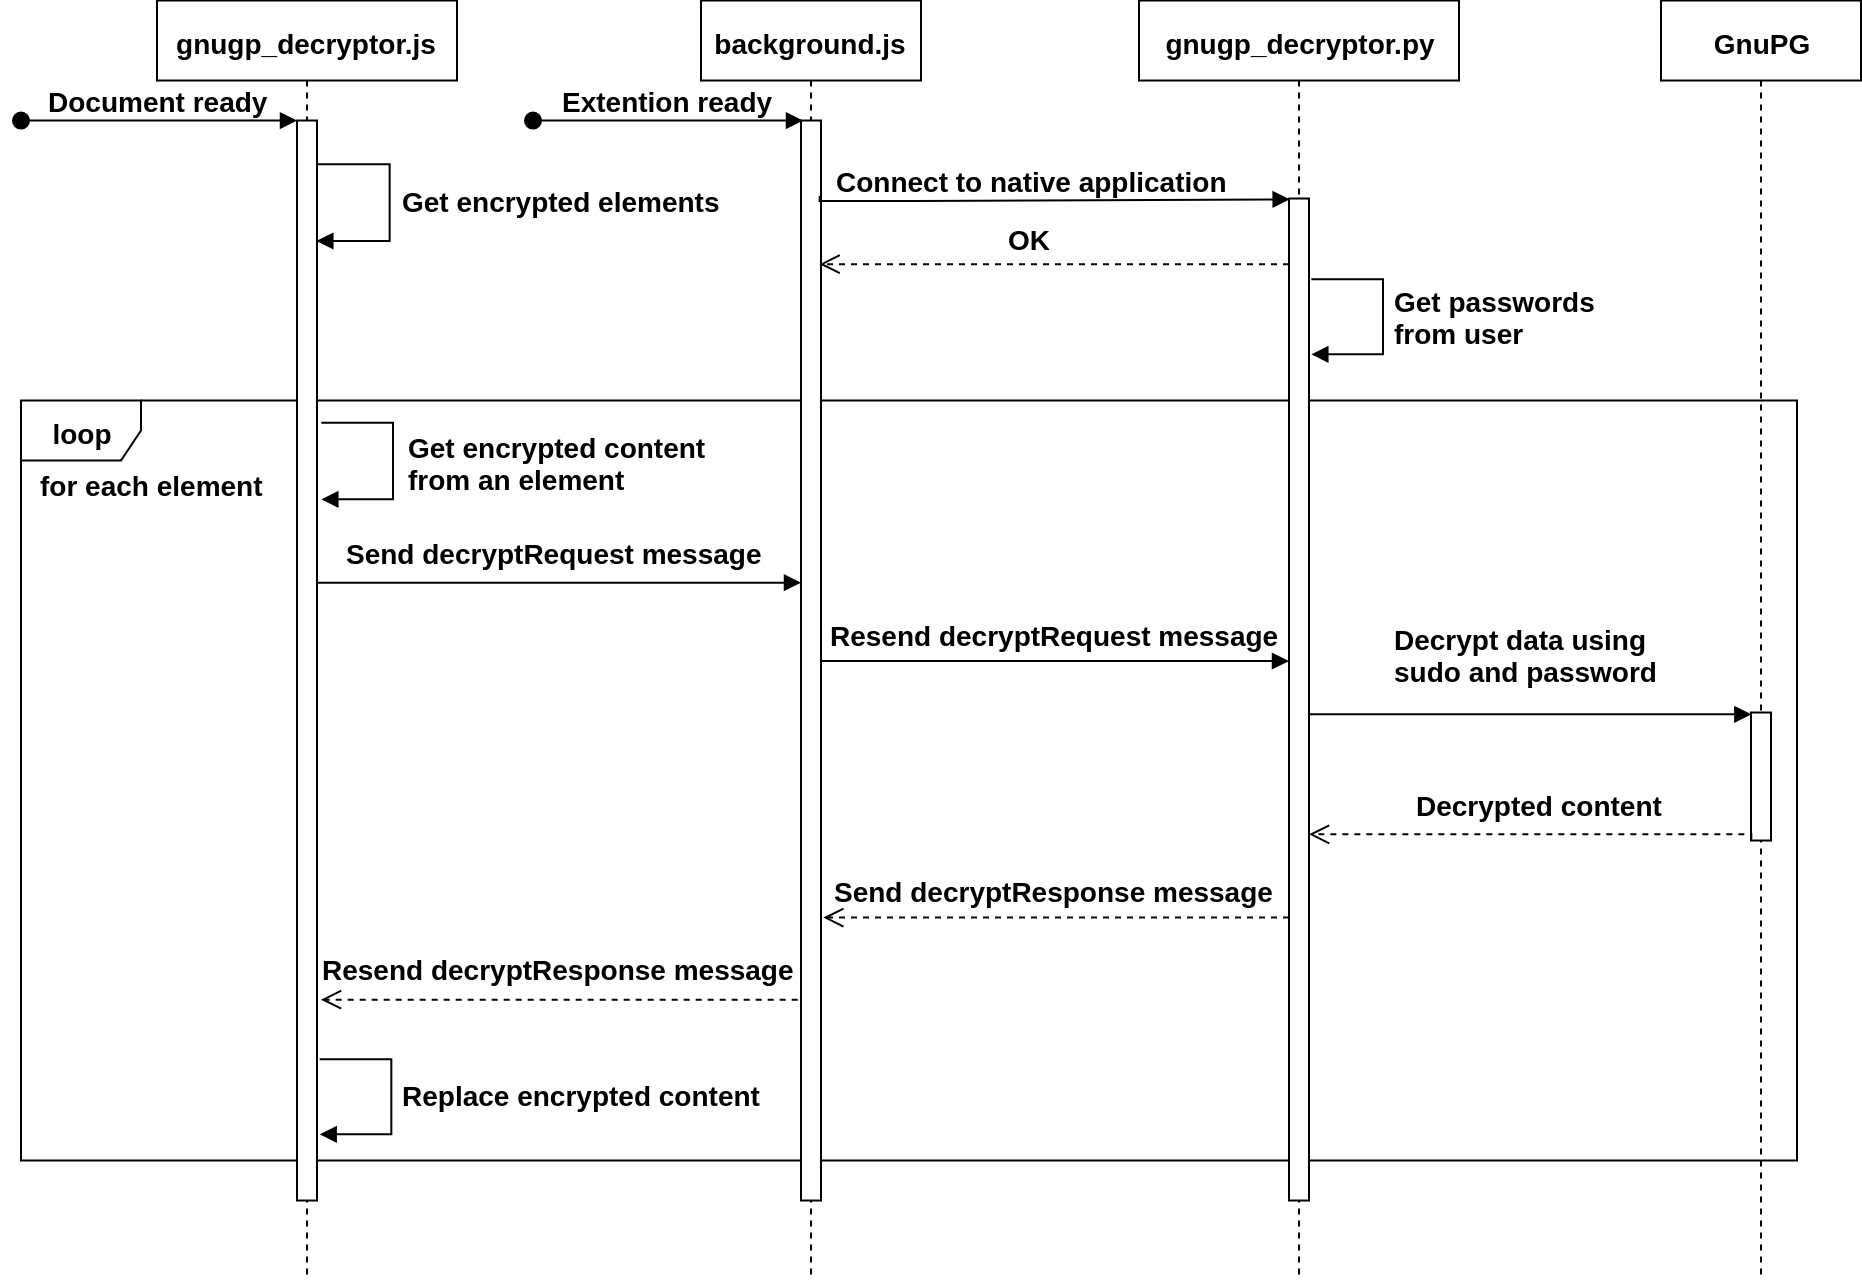
\includegraphics[width=\textwidth]{../obrazky-figures/sequence-gnupg_decryptor.png}
\end{frame}

\begin{frame}
    \frametitle{Zasílání zpráv}
    \textbf{Druhy zpráv:}
    \begin{itemize}
        \item Žádost o dešifrování obsahu -- \textit{decryptRequest}
        \item Odpověď na žádost o dešifrování obsahu -- \textit{decryptResponse}
        \item Ladící zprávy -- \textit{debug}
        \item Informace o chybě v nativní aplikaci -- \textit{error}
        \item Žádost a navázání nového spojení -- \textit{reconnectRequest}
    \end{itemize}
    \medskip
    \textbf{Omezení nativní aplikace:}
    \begin{itemize}
        \item Maximální velikost jedné zprávy je 1\,MB
        \item Celková velikost přenesených dat jsou 4\,GB
    \end{itemize}
\end{frame}

\begin{frame}
    \frametitle{Detekce zašifrovaných prvků}
    \begin{itemize}
        \item Detekce tzv. \czuv{Armoured} textu
        \item Koncovky souborů v \textit{src} atributech
    \end{itemize}
    \medskip
    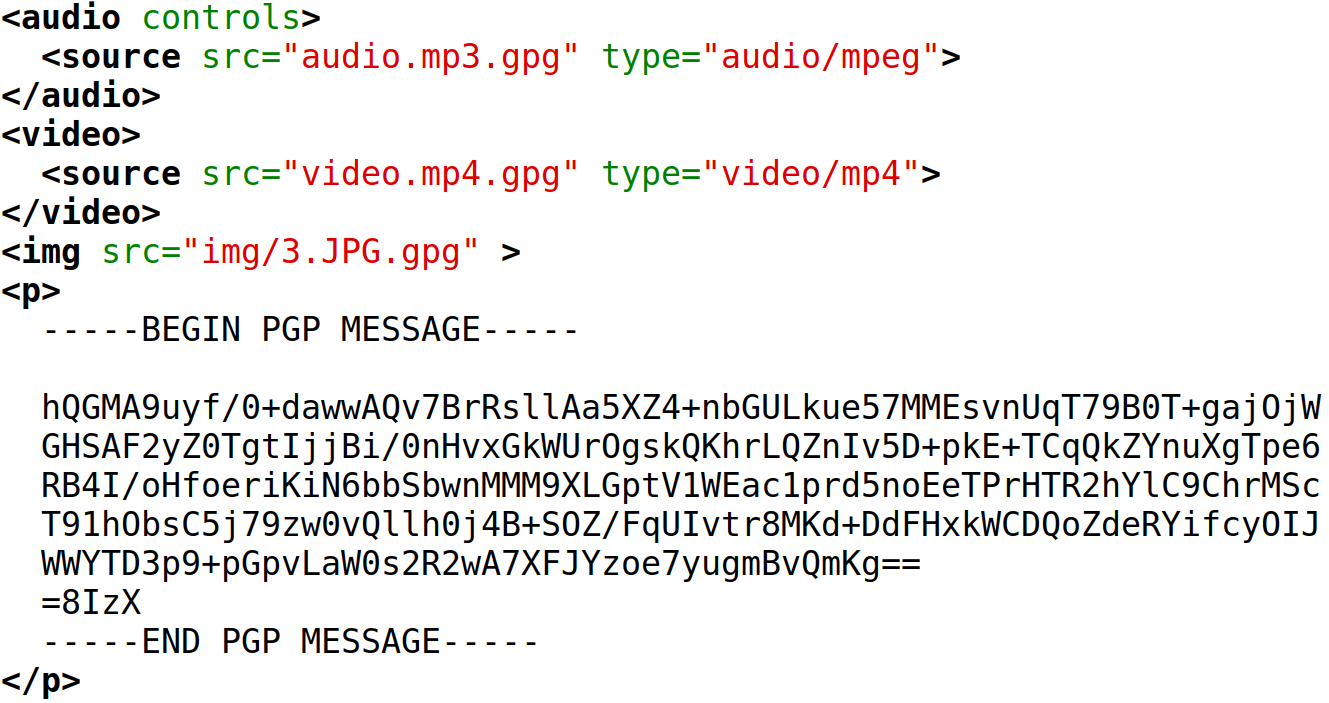
\includegraphics[height=0.6\textheight,keepaspectratio]{img/encrypted.png}
\end{frame}

\begin{frame}
    \frametitle{Interaktivní úpravy stránky}
    \textbf{Problémy s měnícím se DOM stránky:}
    \begin{itemize}
        \item Jiná rozšíření
        \item JavaScript
        \item XHR API
        \item Fetch API
        \item Push API
    \end{itemize}
    \medskip
    Řešení? -- \textbf{MutationObserver}
\end{frame}

\begin{frame}
    \frametitle{Aktuální stav}
    \textbf{Dva implementované prototypy:}
    \begin{itemize}
        \item OpenPGP.js prototype
        \item GnuPG\_Decryptor prototype
    \end{itemize}
    \medskip
    \textbf{Implementované základy:}
    \begin{itemize}
        \item Detekce obrázků
        \item Zasílání zašifrovaných dat nativní aplikaci
        \item Dešifrování dat pomocí GPG
        \item Zobrazení dešifrovaných obrázků
    \end{itemize}
\end{frame}

\begin{frame}
    \frametitle{Budoucí vývoj}
    \textbf{Aktuálně vyvýjený prototyp:}
    \begin{itemize}
        \item Detekce všech zašifrovaných prvků stránky
        \item Rozdělení dat na bloky při překročení maximální velikosti jedné zprávy
    \end{itemize}
    \medskip
    \textbf{Následující prototypy:}
    \begin{itemize}
        \item Kontrola limitu velikosti přenesených dat nativní aplikaci (4\,GB)
        \item Interaktivní úpravy stránky
        \item User interface
        \item Řešení chybových stavů
    \end{itemize}
\end{frame}

\bluepage{Děkuji za pozornost.}

% Questions
\appendix
\addtocounter{framenumber}{-\value{framenumber}} % Framennumber reset

\end{document}
